%% This classfile tries to implement the lay-out of the beamer style beamerthemekuleuven2. This .sty-file can be downloaded here: https://www.kuleuven.be/communicatie/marketing/templates/presentatiemateriaal/index.html Not all options of the style are implemented in this class, for its purpose is merely to mimic the lay-out, and to provide a way to change the lay-out of presentations that were made using the "old" kulakbeamer class. For new documents, we recommend using the .sty-file instead.

\documentclass
   [kulak] % options: kul or kulak (default), handout 
   {kulakbeamer}

\usepackage[dutch]{babel}
\usepackage[utf8]{inputenc}
\usepackage[T1]{fontenc}
\usepackage{textcomp}
\usepackage{siunitx}
\usepackage{subcaption}

\title[HPE]{Human Pose Estimation met OpenPose:}
\subtitle{een toepassing}
\author[Korte naam]{Mathieu Vanooteghem, Isaac Venus \\ 
	en Stan vanhecke} 
\institute[Kulak]{KU Leuven Kulak}
\date{Academiejaar 2020 -- 2021}

%% Overview at begin of each section; delete if unwanted.

\AtBeginSection[]{
	\begin{frame}
	\frametitle{Overzicht} %Change to "Outline" for English presentation
	{
		\hypersetup{hidelinks} %disable link colors
		\hfill	{\large\parbox{.95\textwidth}{\tableofcontents[currentsection,hideothersubsections]}}
	}
\end{frame}}

\begin{document}

\begin{titleframe}
\titlepage
\end{titleframe}

\begin{outlineframe}[Overzicht]
\tableofcontents
\end{outlineframe}

 % % % Here you go  % % % 

\section{Inleiding}

\begin{frame}
\frametitle{Inleiding}
	\begin{itemize}
		\item stevig prijskaartje aan medische toepassingen
		\item werken met alledaagse technologie
		\item HPE: schatten van lichaamspositie
		\item verschillende toepassingen
	\end{itemize}
\end{frame}



\section[Korte titel]{Theoretische achtergrond}

\begin{frame}
\frametitle{HPE, revolutionair?}
\begin{center}
	\begin{tabular}{l|l} 
		\textbf{3D motion capture pak} & \textbf{Human pose estimation}\\
		\hline
		- veel rekenkracht & + HPE mogelijk met gewone laptop\\
		- hoogtechnologische apparatuur & + alleen laptop en camera nodig\\
		- mensen ter plaatse aanwezig & + vanop afstand via foto of video\\
		+ heel precieze & - ruwe schatting van \\
		  lichaamspositiebepaling & lichaamspositie\\
	\end{tabular}
\end{center}
\end{frame}

\begin{frame}
\frametitle{Werking van Openpose: Bepalen van de lichaamspositie}

\begin{center}
	\begin{tabular}{l|l} 
		\textbf{Top-down aanpak} & \textbf{Bottom-up aanpak}\\
		\hline
		1. personendetector & 1. belangrijke knooppunten bepalen\\
		2. pose schatten per persoon & 2. punten op juiste manier linken\\
		& => poses bepalen\\
		\hline
		- runtime \textasciitilde \#personen  & + veel efficiënter dan Top-down\\
		- fout in stap 1 niet goed  & \\
		 te maken in stap 2 & \\
	\end{tabular}
\end{center}
\end{frame}

\begin{frame}
	nog iets over part affinity fields en heatmaps??
	\begin{figure}
		\centering
		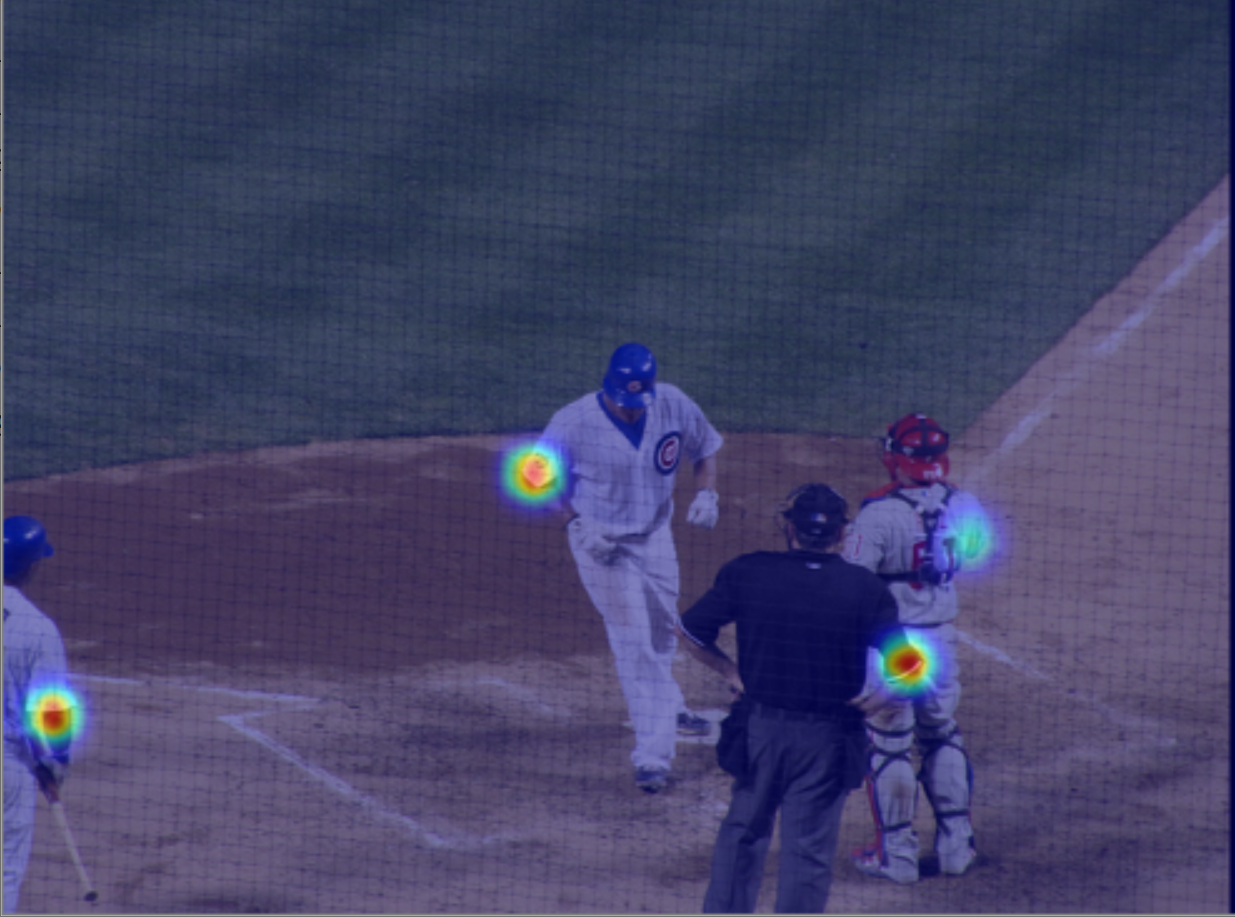
\includegraphics[width=0.5\textwidth]{heatmap_1}
	\end{figure}
\end{frame}

\section{Toepassing 1: Opvolgen van revalidatie na schouderoperatie}

\begin{frame}
\frametitle{Bepalen van de hoek tussen arm en borst}
\begin{itemize}
	\item hoek tussen [32] en [21] of [15] en [56]
	\item m.b.v. cosinusregel via coördinaten
\end{itemize}
\begin{figure}
	\centering
	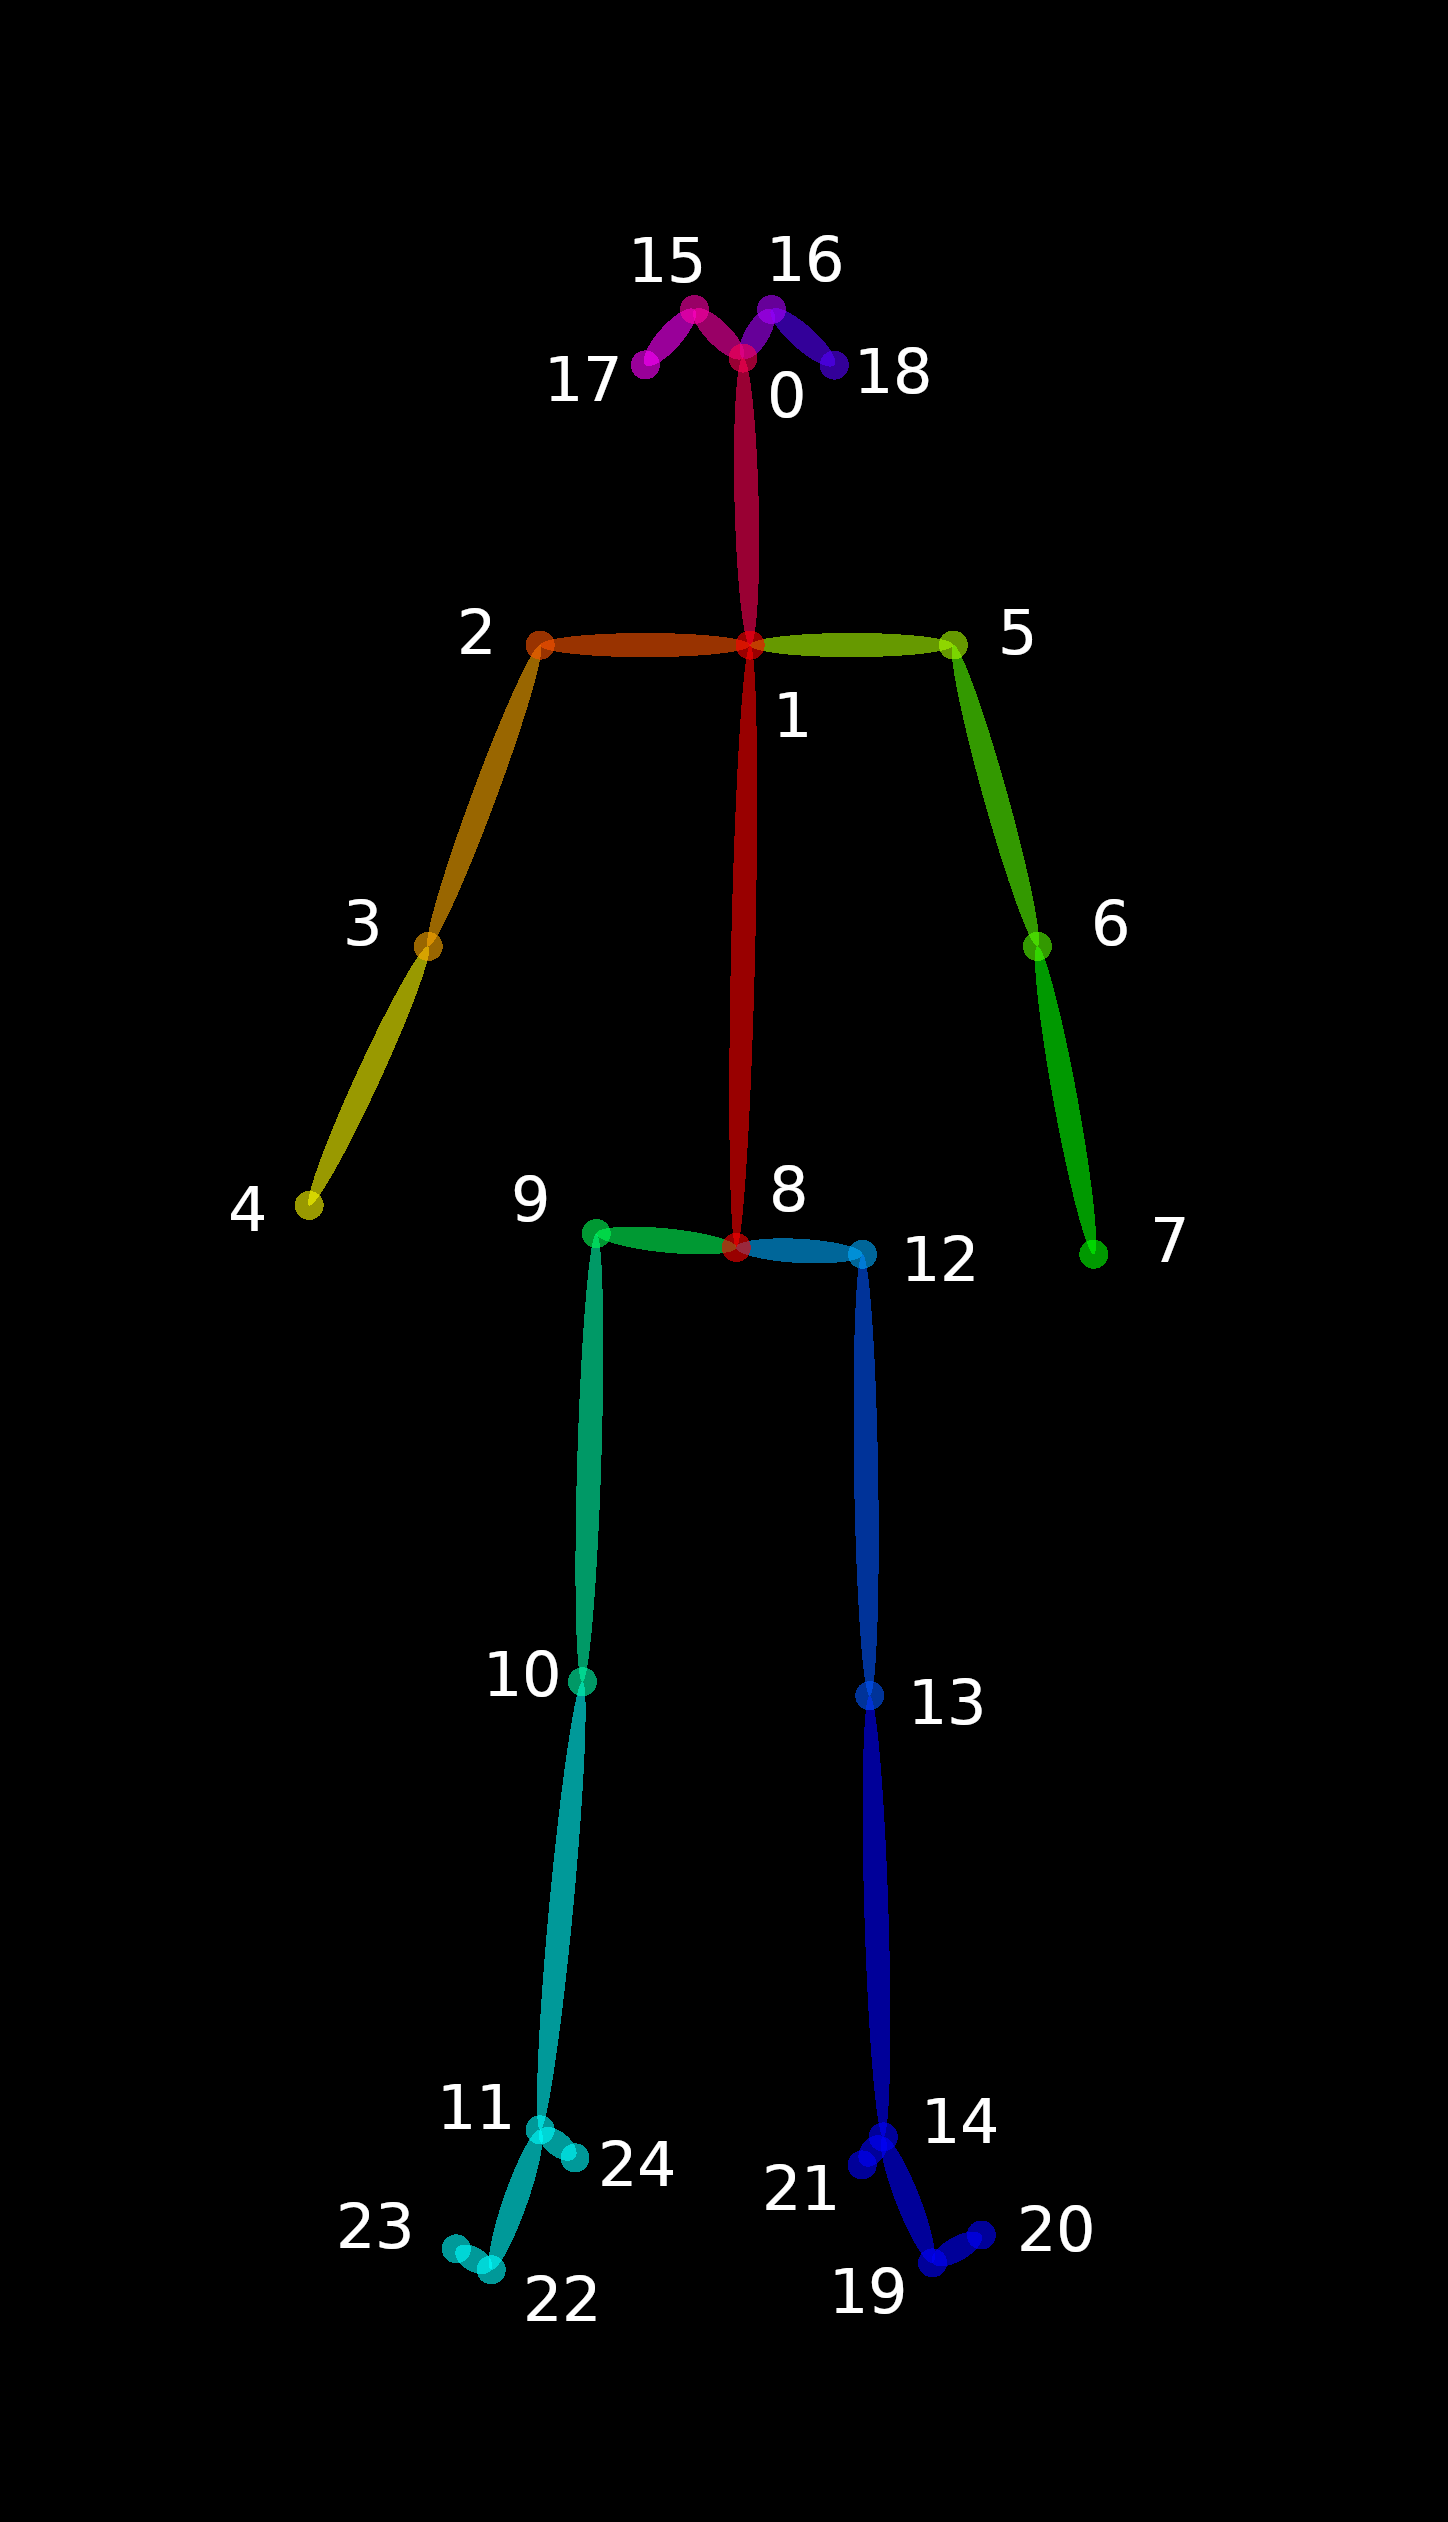
\includegraphics[width= .3\textwidth]{HPE_skelet}
\end{figure}
\end{frame}

\begin{frame}
\frametitle{Resultaten en conclusies}
\begin{itemize}
	\item foto recht nemen (Openpose werkt in 2D)
	\item telkens vanuit zelfde positie om revalidatie te evalueren
\end{itemize}
\end{frame}



\section{Toepassing 2: Fietspositie bepalen}

\begin{frame}
	\frametitle{Wat is een bikefit?}
	\begin{itemize}
		\item analyseren van de positie op de fiets
		\item eventuele aanpassingen voorstellen obv analyse
		\item doel: blessurepreventie en aerodynamica
	\end{itemize}
\begin{figure}
	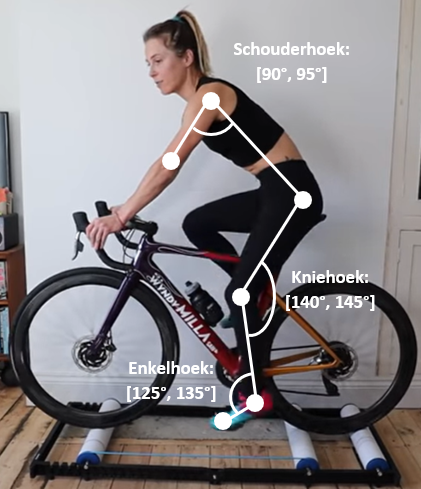
\includegraphics[width= .4\textwidth]{bikefit_hoeken_foto}
\end{figure}
\end{frame}

\begin{frame}
	\frametitle{Algoritme voor het wijzigen van de zadelhoogte}
	\begin{itemize}
		\item vooral zadelhoogte beïnvloedt kniehoek
		\item kniehoek moet tussen 140° en 145°
		\item wijziging van zadelhoogte met aantal pixels
		\item pixels --> \si{cm}
	\end{itemize}
\end{frame}

\begin{frame}
	\frametitle{Algoritme voor het wijzigen van de stuurpenlengte}
	\begin{itemize}
		\item vooral stuurpenlengte beïnvloedt schouderhoek
		\item beschikbaar in lengte van 40 tot 140 \si{mm}
		
	\end{itemize}
\end{frame}

\begin{frame}
	\frametitle{Conclusies}
	\begin{itemize}
		\item invloed van de resolutie
		\item pose is slechts een schatting van Openpose
		\item fouten op omzetting van pixels naar \si{cm}
		\item probleem met rug bij bepalen schouderhoek
	\end{itemize}

	Besluit: Bikefitting is heel precieze wetenschap <-> Openpose maakt slechts schatting
\end{frame}

\begin{frame}
	\frametitle{Demonstratie}
	\begin{figure}
		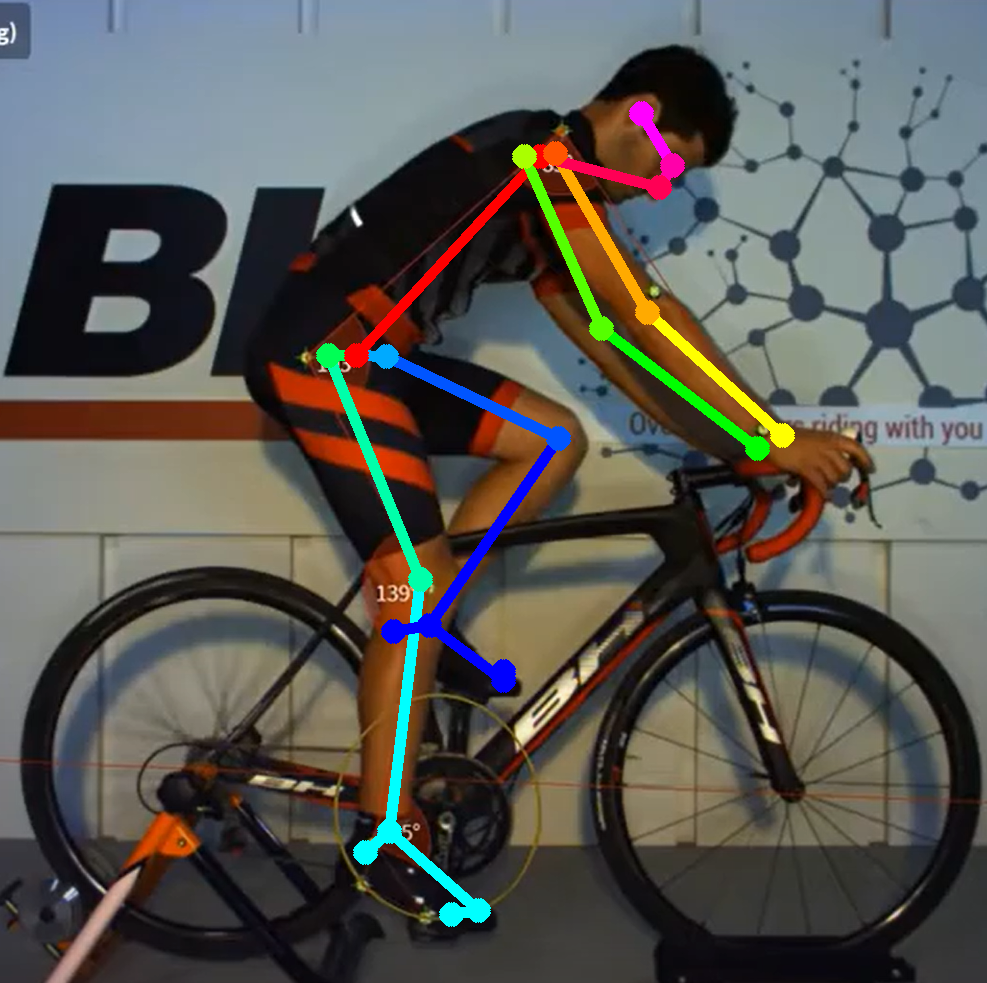
\includegraphics[width= .55\textwidth]{prof_bikefit}
	\end{figure}
\end{frame}



\section{Toepassing 3: Correct uitvoeren van fitnessoefeningen}

\begin{frame}
	\frametitle{Richtlijnen voor een goeie squat}
	1. Knie boven de tenen
	\begin{figure}
		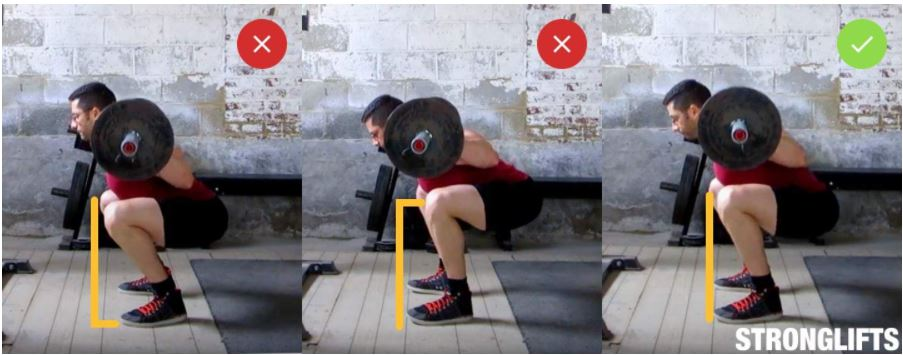
\includegraphics[width= \textwidth]{squat_knie}
	\end{figure}
\end{frame}

\begin{frame}
\frametitle{Richtlijnen voor een goeie squat}
2. Heup op dezelfde hoogte als knie
\begin{figure}
	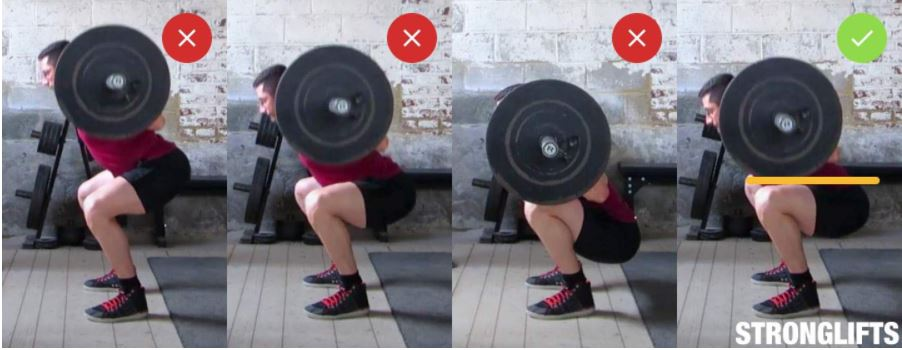
\includegraphics[width= \textwidth]{squat_heup}
\end{figure}
\end{frame}

\begin{frame}
	\frametitle{Conclusies}
	\begin{itemize}
		\item komt niet aan op millimeters
		\item beter geschikt voor Openpose
	\end{itemize}
\end{frame}

\begin{frame}
	\frametitle{Demonstratie}
	\begin{figure}
		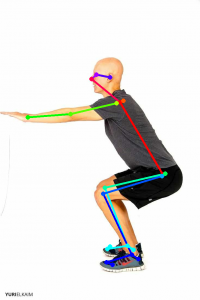
\includegraphics[width= .4\textwidth]{squat_HPE}
	\end{figure}
\end{frame}



\section{Besluit}

\begin{frame}
\frametitle{Besluit}
\begin{itemize}
	\item niet geschikt voor medische toepassingen
	\item wel voor minder precieze doeleinden
	% Minder relevant maar ik wil dit er toch graag eens bij vermelden
	\item bijzonder moeilijke installatie
\end{itemize}
\end{frame}

\section*{Einde}
\begin{frame}
\frametitle{Einde}
\begin{center}
	Bedankt voor het luisteren\\
	Zijn er nog vragen?
\end{center}
\end{frame}
\end{document}
